\documentclass[xcolor=table,dvipsnames,svgnames,aspectratio=169,fontset=ubuntu]{ctexbeamer}
% 可以通过 fontset=macnew / fontset=ubuntu / fontset=windows 选项切换字体集
\usepackage{tikz}
\usepackage[normalem]{ulem}
\usetikzlibrary{arrows}
\usepackage{amsmath}
\usepackage{mflogo}
\usepackage{graphicx}
\usepackage{ccicons}
\usepackage{hologo}
\usepackage{colortbl}
\usepackage{shapepar}
\usepackage{hyperxmp}
\usepackage{booktabs}
\usepackage{qrcode}
\usepackage{listings}
\usepackage{tipa}
\usepackage{multicol}
\usepackage{datetime2}
\usepackage{fontawesome5}
\usepackage{hyperref}
\usepackage{enumitem}
\usepackage{bm}
\usepackage[backend=biber,style=gb7714-2015]{biblatex}
\addbibresource{thesis.bib}
\graphicspath{{figures/}}
\hypersetup{
  pdfsubject = {上海交通大学图书馆专题培训讲座},
  pdfauthor = {Alexara Wu},
  pdfcopyright = {Licensed under CC-BY-SA 4.0. Some rights reserved.},
  pdflicenseurl = {http://creativecommons.org/licenses/by-sa/4.0/},
  unicode = true,
  psdextra = true,
  pdfdisplaydoctitle = true
}

\DeclareOptionBeamer{en}

\pdfstringdefDisableCommands{
  \let\\\relax
  \let\quad\relax
  \let\hspace\@gobble
}
\renewcommand{\TeX}{\hologo{TeX}}
\renewcommand{\LaTeX}{\hologo{LaTeX}}
\newcommand{\BibTeX}{\hologo{BibTeX}}
\newcommand{\XeTeX}{\hologo{XeTeX}}
\newcommand{\pdfTeX}{\hologo{pdfTeX}}
\newcommand{\LuaTeX}{\hologo{LuaTeX}}
\newcommand{\MiKTeX}{\hologo{MiKTeX}}
\newcommand{\MacTeX}{Mac\hologo{TeX}}
\newcommand{\beamer}{\textsc{beamer}}
\newcommand{\XeLaTeX}{\hologo{Xe}\kern-.13em\LaTeX{}}
\newcommand{\pdfLaTeX}{pdf\LaTeX{}}
\newcommand{\LuaLaTeX}{Lua\LaTeX{}}
\def\TeXLive{\TeX{} Live}
\let\TL=\TeXLive
\newcommand{\SJTUThesis}{\textsc{SJTUThesis}}
\newcommand{\SJTUThesisVersion}{1.1.0}
\newcommand{\SJTUThesisDate}{2023/3/24}
\newcommand{\SJTUBeamer}{\textsc{SJTUBeamer}}
\newcommand{\SJTUBeamerVersion}{3.0.0}
\newcommand{\SJTUBeamerDate}{2022/11/22}
\newcommand\link[1]{\href{#1}{\faLink}}
\newcommand\pkg[1]{\texttt{#1}}
\def\cmd#1{\texttt{\color{structure}\footnotesize $\backslash$#1}}
\def\env#1{\texttt{\color{structure}\footnotesize #1}}
\def\cmdxmp#1#2#3{\small{\texttt{\color{structure}$\backslash$#1}\{#2\}
\hspace{1em}\\ $\Rightarrow$\hspace{1em} {#3}\par\vskip1em}}
\lstset{
  language=[LaTeX]TeX,
  basicstyle=\ttfamily\footnotesize,
  tabsize=2,
  keywordstyle=\bfseries\ttfamily\color{cprimary},
  commentstyle=\sl\ttfamily\color[RGB]{100,100,100},
  stringstyle=\ttfamily\color[RGB]{50,50,50},
  extendedchars=true,
  breaklines=true,
}

\usetheme[maxplus,blue,smoothbars]{sjtubeamer}
% 使用 maxplus/max/min 切换标题页样式
% 使用 red/blue 切换主色调
% 使用 light/dark 切换亮/暗色模式
% 使用外样式关键词以获得不同的边栏样式
%   miniframes infolines  sidebar
%   default    smoothbars split	 
%   shadow     tree       smoothtree
% 使用 topright/bottomright 切换徽标位置
% 使用逗号分隔列表以同时使用多种选项

\author{上海交通大学学生创新中心}
\date{\the\year \,.\the\month \,}
%\subject{LaTeX, 论文排版, SJTUThesis}
\title[流形上的Soblev不等式与嵌入]
{\textnormal{黑盒优化与启发式算法}} 

\setbeamercolor{block title alerted}{use=structure,fg=white,bg=structure.fg!88!black}
\setbeamercolor{block body alerted}{parent=normal text,use=block title,bg=block title.bg!10!white}


%=================================================================
%==================================================================

\begin{document}

\maketitle
%-----------------------------------------------------------------------
\section{黑盒优化与启发式算法}
\begin{frame}{黑盒优化}
  黑盒优化问题泛指目标函数难以从数学上解析表达,缺少可直接利用的梯度信息,仅可利用目标函数输入和对应输出函数值进行最优解搜索的优化问题。
  \vskip 20pt
  \begin{figure}
    \centering
    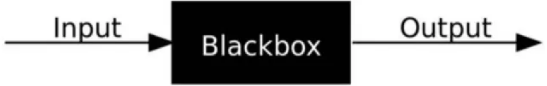
\includegraphics[width=0.6\textwidth]{黑盒优化.png}
  \end{figure}
\end{frame}

\begin{frame}{启发式算法}
  启发式算法是一种基于直观或经验构造的算法,它不是通过完全遍历所有可能的解决方案来找到最佳解决方案,而是依赖于对问题的理解和一些经验规则来快速找到可能的解决方案。
  
  \vskip 20pt
  这种算法并不能保证找到全局最优解,只能找到局部最优解。

  \vskip 20pt
  常见的启发式算法包括遗传算法、蚁群算法、模拟退火算法等。
\end{frame}



\section{粒子群算法}
\begin{frame}{粒子群算法简介}
  粒子群优化(PSO)算法由 James Kennedy 等人于 1995
年提出,提出该算法的灵感来自动物界中鸟群、兽群和鱼群等的迁移、捕食等群体活动。
在群体活动中,每一个个体都会受益于所有成员在这个过程中发现和累积的经验,因此粒子群算法属于启发式算法的一种。
\vskip 10pt
粒子群优化算法原理简单,在内存需求和计算速度方面的成本较低,是一种能够优化
非线性和多维问题的算法。该算法的基本概念是构造一群粒子,粒子群在其周围的空间(也
就是问题空间)中移动,寻找它们的目标点。

\end{frame}

\begin{frame}{粒子群算法原理}
  假设在一个 $D$ 维的目标搜索空间中,有 $N$ 个粒子组成一个群落,其中第 $i$ 个粒子表示为一个 $D$ 维的向量:
$$
X_i=\left(x_{i 1}, x_{i 2}, \cdots, x_{i D}\right), \quad i=1,2, \cdots, N
$$

第 $i$ 个粒子的“飞行”速度也是一个 $D$ 维的向量,记为:
$$
V_i=\left(v_{i 1}, v_{i 2}, \cdots, v_{i D}\right), \quad i=1,2, \cdots, N
$$
\end{frame}

\begin{frame}{粒子群算法原理}
  第 $i$ 个粒子迄今为止搜索到的最优位置称为个体极值,记为:
$$
P_{\text {best }}=\left(p_{i 1}, p_{i 2}, \cdots, p_{i D}\right), \quad i=1,2, \cdots, N
$$

整个粒子群迄今为止搜索到的最优位置为全局极值,记为:
$$
g_{\text {best }}=\left(g_1, g_2, \cdots, g_D\right)
$$
\end{frame}

\begin{frame}{粒子群算法原理}
  在找到这两个最优值时,粒子根据如下的式子来更新自己的速度和位置:
$$
\begin{aligned}
  v_{i j}(t+1)&=v_{i j}(t)+c_1 r_1(t)\left[p_{i j}(t)-x_{i j}(t)\right]+c_2 r_2(t)\left[p_{g j}(t)-x_{i j}(t)\right] \\
  x_{i j}(t+1)&=x_{i j}(t)+v_{i j}(t+1)\\
\end{aligned}
$$

其中 : $c_1$和$c_2$为学习因子,也称加速常数 ; $r_1$ 和 $r_2$ 为 $[0,1]$ 范围内的均匀随机数,增加了粒子飞行的随机性 ; $v _{i j}$ 是粒子的速度,$v_{ij} \in [-v_{max}, v_{max}]$,$v_{max}$是常数,由用户设定来限制粒子的速度。
\vskip 10pt
式 (1) 等号右侧可以分为三部分:“惯性”+“认知”+“社会”。
\end{frame}

\begin{frame}{粒子群算法流程}
\begin{columns}
\column{0.8\textwidth}
(1)初始化粒子群:群体规模  $N$,每个粒子的位置 $x_i$ 和速度 $v_i$。 

(2)计算每个粒子的适应度值 $fit[i]$。 

(3)对每个粒子,用它的适应度值 $fit[i]$ 和个体极值 $p_{best}(i)$ 比较。

\qquad 如果 $fit[i] > p_{best}(i)$,则用 $fit[i]$替换掉 $p_{best}(i)$。 

(4)对每个粒子,用它的适应度值 $fit[i]$ 和全局极值 $g_{best}$ 比较。

\qquad 如果 $fit[i] > g_{best}$ 则用 $fit[i]$替换掉 $g_{best}$。 

(5)迭代更新粒子的速度 $v_i$ 和位置 $x_i$。 

(6)进行边界条件处理。

(7)判断算法终止条件是否满足:若是,则结束;否则返回步骤(2)。
\column{0.2\textwidth}
\begin{figure}
  \centering
  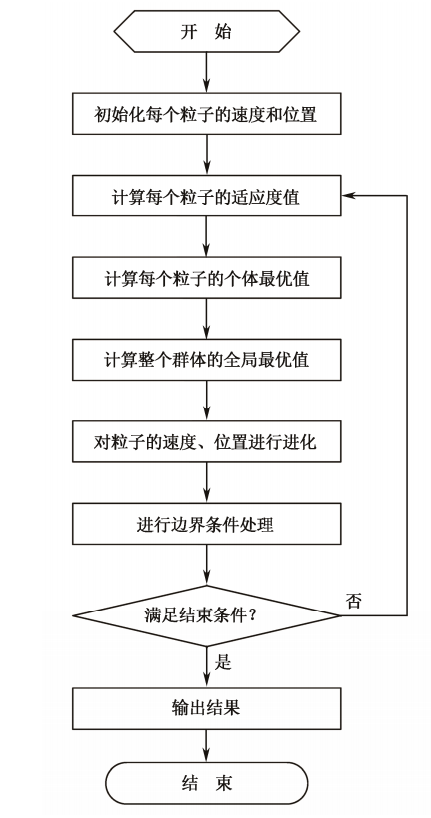
\includegraphics[width=\textwidth]{粒子群.png}
\end{figure}
\end{columns}
\end{frame}

\begin{frame}{粒子群算法求解优化问题}
  \begin{columns}
    \column{0.65\textwidth}
    【例1】
    \vskip 10pt
    求函数 \(f(x,y) = 3cos(xy) + x + y^2\) 的最小值,其中 \(x\) 的取值范围为\([-4,4]\),\(y\) 的取值范围为\([-4,4]\)
  

    \column{0.4\textwidth} 
    \begin{figure}
      \centering
      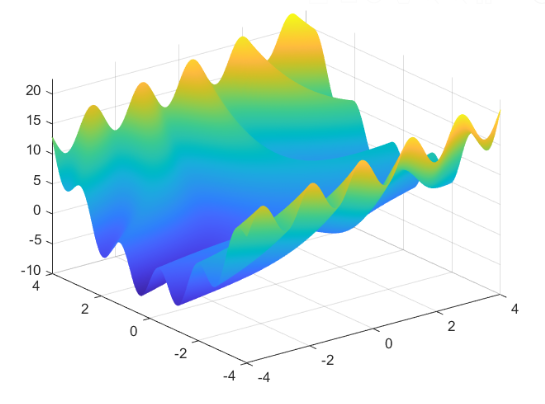
\includegraphics[width=\textwidth]{例1.png}
    \end{figure}
  \end{columns}
\end{frame}




\section{遗传算法}
\begin{frame}{遗传算法简介}
  \begin{columns}
  \column{0.4\textwidth}
  遗传算法(Genetic Algorithms)是一种基于自然选择原理和自然遗传机
  制的搜索算法,它是模拟自然界中的生命进化机制,在人工系统中实现特定目
  标的优化。
  \column{0.5\textwidth}
  \begin{figure}
    \centering
    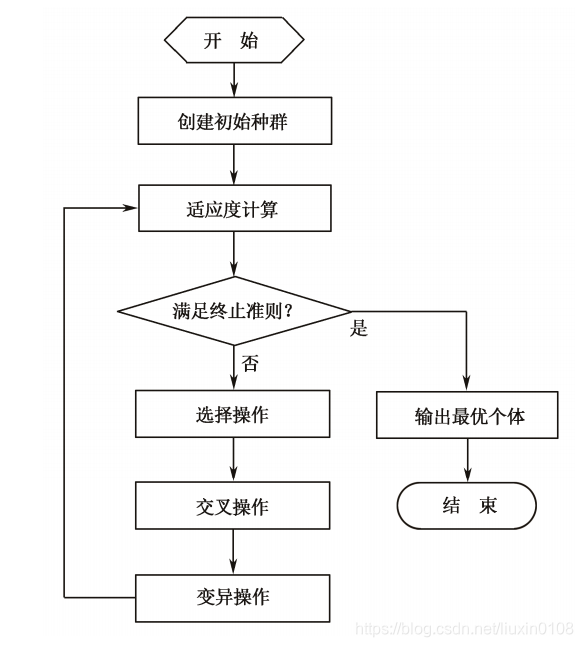
\includegraphics[width=0.8\textwidth]{遗传算法.png}
  \end{figure}
  \end{columns}
\end{frame}

\begin{frame}{遗传算法原理}
  Step1. 根据具体问题确定可行解域,确定一种编码方法,能用数值串或字符串\\
  
  \qquad\quad\; 表示可行解域的每一解。

  \vskip 15pt
  Step2. 对每一解应有一个度量好坏的依据,它用一函数表示,叫做适应度函数

  \vskip 15pt
  Step3. 确定进化参数群体规模 $M$ 、交叉概率 $P_c$ 、变异概率 $P_m$ 、进化终止条件
\end{frame}

\begin{frame}{遗传算法原理}
  \begin{columns}
    \column{0.6\textwidth}
    \begin{figure}
      \centering
      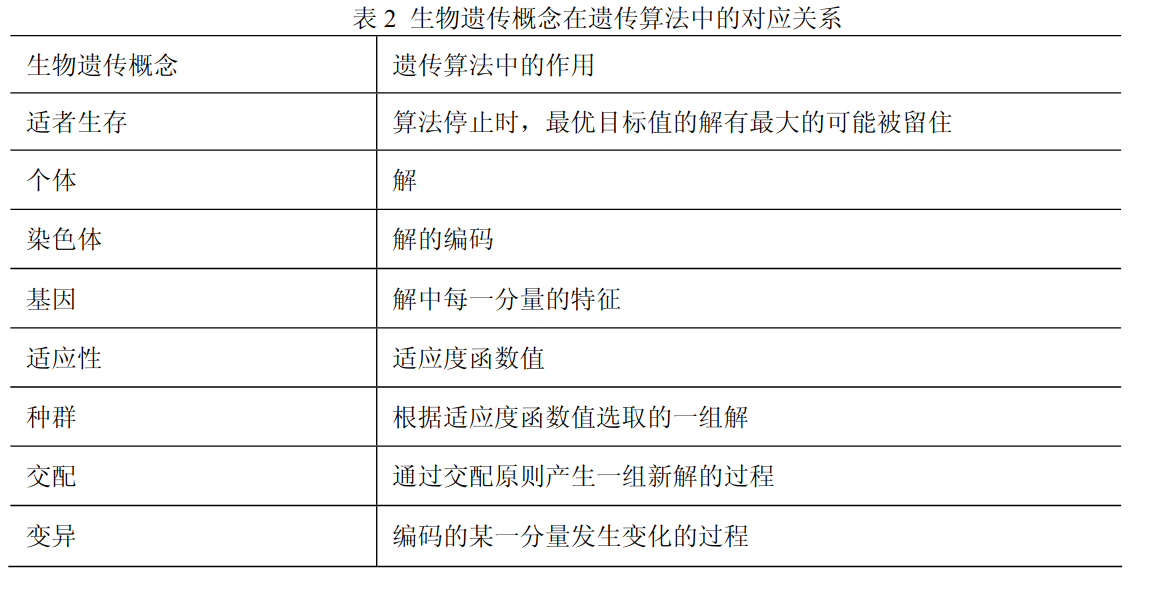
\includegraphics[width=\textwidth]{遗传算法对应.png}
    \end{figure}
    \column{0.5\textwidth}
    \begin{figure}
      \centering
      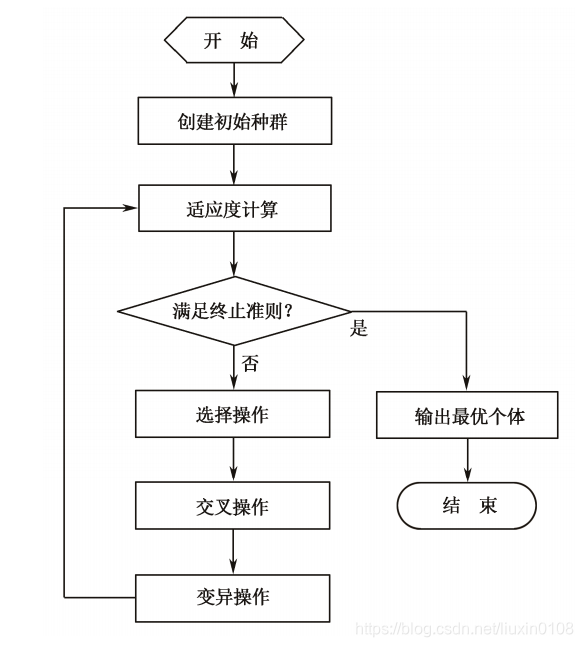
\includegraphics[width=0.8\textwidth]{遗传算法.png}
    \end{figure}
    \end{columns}
\end{frame}

\begin{frame}{遗传算法求解优化问题}
  \begin{columns}
    \column{0.5\textwidth}、
    \begin{figure}
      \centering
      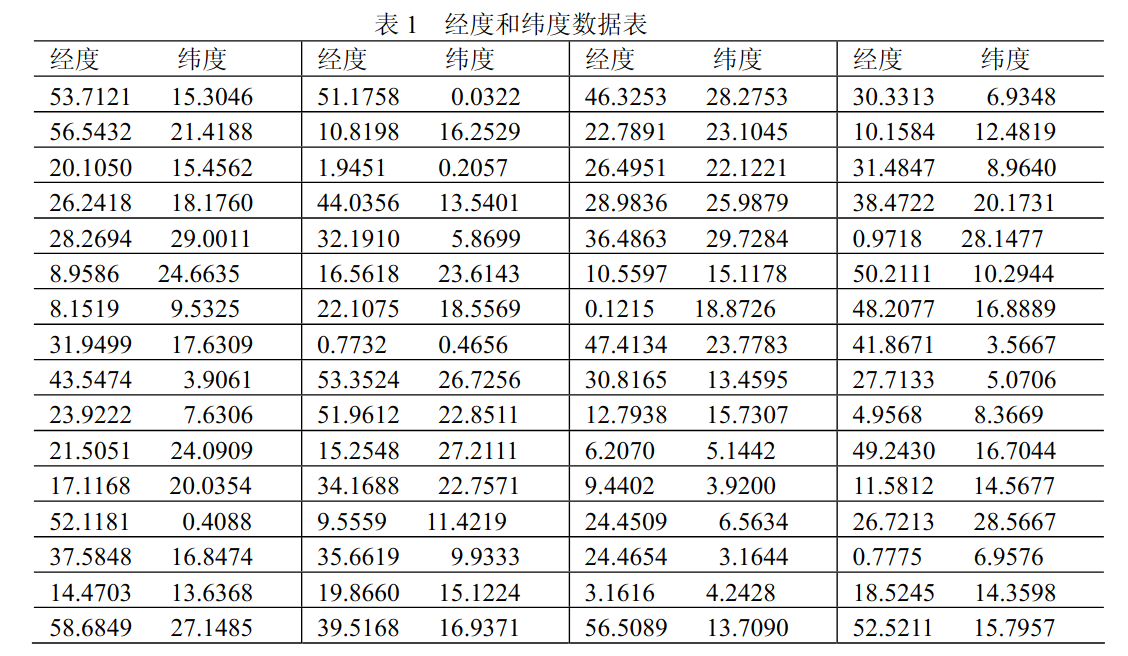
\includegraphics[width=\textwidth]{例1-1.png}
    \end{figure}
    \column{0.5\textwidth} 
    【例2】
    \vskip 10pt
    已知敌方 100 个目标的经纬度如表 1 所示   
    \begin{figure}
      \centering
      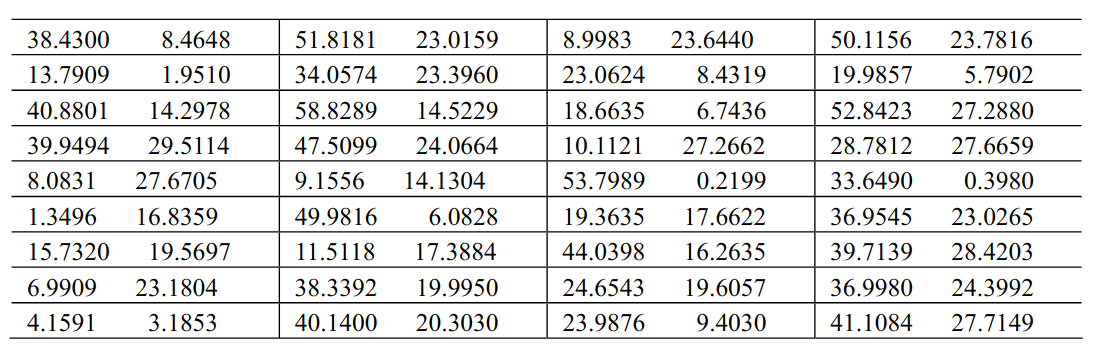
\includegraphics[width=\textwidth]{例1-2.png}
    \end{figure}
  \end{columns}
\end{frame}

\begin{frame}{遗传算法求解优化问题}
  【例2】我方有一个基地,经度和纬度为(70,40)。假设我方飞机的速度为 1000 公里/小时。
  我方派一架飞机从基地出发,侦察完敌方所有目标,再返回原来的基地。在敌方每一目
  标点的侦察时间不计,求该架飞机所花费的时间(假设我方飞机巡航时间可以充分长)。
\end{frame}

\begin{frame}{遗传算法求解例2}
  我们依次给基地编号为 1,敌方目标依次编号为 2,3,…,101,最后我方基地再重复编号为 102(这样便于程序中计算)

  \vskip 10pt
  上面问题中给定的是地理坐标 (经度和纬度), 我们必须求两点间的实际距离。设 $A, B$ 两点的地理坐标分别为 $\left(x_1, y_1\right),\left(x_2, y_2\right)$, 过 $A, B$ 两点的大圆的劣弧长即为两点的实际距离。以地心为坐标原点 $O$, 以赤道平面为 $X O Y$ 平面, 以 0 度经线圈所在的平面为 $X O Z$ 平面建立三维直角坐标系。则 $A, B$ 两点的直角坐标分别为:
  $$
  \begin{aligned}
  & A\left(R \cos x_1 \cos y_1, R \sin x_1 \cos y_1, R \sin y_1\right) \\
  & B\left(R \cos x_2 \cos y_2, R \sin x_2 \cos y_2, R \sin y_2\right)
  \end{aligned}
  $$
  
  其中 $R=6370$ 为地球半径。
\end{frame}

\begin{frame}{遗传算法求解例2}
  $A, B$ 两点的实际距离
$$
d=R \arccos \left(\frac{\overrightarrow{\mathrm{OA}} \cdot \overrightarrow{O B}}{|\overrightarrow{\mathrm{OA}}| \cdot|\overrightarrow{O B}|}\right),
$$

化简得
$$
d=R \arccos \left[\cos \left(x_1-x_2\right) \cos y_1 \cos y_2+\sin y_1 \sin y_2\right] 
$$
\end{frame}

\begin{frame}{遗传算法求解例2}
  求解例2的遗传筫法的参数设定如下:

  \vskip 8pt
  种群大小: $M=50$

  \vskip 8pt
  最大代数: $G=1000$

  \vskip 8pt
  交叉率: $p_c=1$, 交叉概率为 1 能保证种群的充分进化。

  \vskip 8pt
  变异率: $p_m=0.1$, 一般而言, 变异发生的可能性较小。
\end{frame}

\begin{frame}{遗传算法求解例2}
  (1)编码策略

  \vskip 5pt
  采用十进制编码, 用随机数列 $\omega_1 \omega_2 \ldots \omega_{102}$ 作为染色体, 其中 
  
  $$0<\omega_i<1,(i=2,3, \cdots, 101), \omega_1=0, \omega_{102}=1$$
  \vskip 5pt
  每一个随机序列都和种群中的一个个体相对应, 例如 9 目标问题的一个染色体为:
  $$
  [0.23,0.82,0.45,0.74,0.87,0.11,0.56,0.69,0.78]
  $$
  
  其中编码位置 $i$ 代表目标 $i$, 位置 $i$ 的随机数表示目标 $i$ 在巡回中的顺序, 我们将这些随机数按升序排列得到如下巡回:
  $$
  6-1-3-7-8-4-9-2-5
  $$
\end{frame}

\begin{frame}{遗传算法求解例2}
  (2)初始种群
  \vskip 5pt
  先利用经典的近似算法一改良圈算法求得一个较好的初始种群。即对于初始圈
  $$
  C=\pi_1 \cdots \pi_{u-1} \pi_u \pi_{u+1} \cdots \pi_{v-1} \pi_v \pi_{v+1} \cdots \pi_{102}, \quad 2 \leq u<v \leq 101, \quad 2 \leq \pi_u<\pi_v \leq 101
  $$
  
  交换 $u$ 与 $v$ 之间的顺序, 此时的新路径为:
  $$
  \pi_1 \cdots \pi_{u-1} \pi_v \pi_{v-1} \cdots \pi_{u+1} \pi_u \pi_{v+1} \cdots \pi_{102}
  $$
  
  记 $\Delta f=\left(d_{\pi_{u-1} \pi_v}+d_{\pi_u \pi_{v+1}}\right)-\left(d_{\pi_{u-1} \pi_u}+d_{\pi_v \pi_{v+1}}\right)$, 若 $\Delta f<0$, 则以新的路经修改旧的路经, 直到不能修改为止。
\end{frame}

\begin{frame}{遗传算法求解例2}
  (3) 目标函数
\vskip 5pt
目标函数为侦察所有目标的路径长度, 适应度函数就取为目标函数。我们要求
$$
\min f\left(\pi_1, \pi_2, \cdots, \pi_{102}\right)=\sum_{i=1}^{101} d_{\pi_i \pi_{i+1}}
$$
(4) 交叉操作
\vskip 5pt
我们的交叉操作采用单点交叉。设计如下, 对于选定的两个父代个体 

$$f_1=\omega_1 \omega_2 \ldots \omega_{102}, f_2=\omega_1^{\prime} \omega_2^{\prime} \ldots \omega_{102}^{\prime}$$
\vskip 5pt
我们随机地选取第 $t$ 个基因处为交叉点, 则经过交叉运算后得到的子代编码为 $s_1$ 和 $s_2, s_1$ 的基因由 $f_1$ 的前 $t$ 个基因和 $f_2$ 的后 $102-t$ 个基因构成, $s_2$ 的基因由 $f_2$ 的前 $t$ 个基因和 $f_1$ 的后 $102-t$ 个基因构成。
\end{frame}

\begin{frame}{遗传算法求解例2}
  例如:
  $$
\begin{aligned}
& f_1=\left[\begin{array}{lllllll}
0, & 0.14, & 0.25, & 0.27, \mid & 0.29, & 0.54, \cdots, 0.19, & 1
\end{array}\right] \\
& f_2=\left[\begin{array}{lllllll}
0, & 0.23, & 0.44, & 0.56, \mid & 0.74, & 0.21, \cdots, 0.24, &1
\end{array}\right] \\
&
\end{aligned}
$$

设交叉点为第四个基因处, 则
$$
\begin{aligned}
& s_1=\left[\begin{array}{lllllll}
0, & 0.14, & 0.25, & 0.27, \mid & 0.74, & 0.21, \cdots, 0.24,&1
\end{array}\right] \\
& s_2=\left[\begin{array}{lllllll}
0, & 0.23, & 0.44, & 0.56, \mid & 0.29, & 0.54, \cdots, 0.19,&1
\end{array}\right] \\
&
\end{aligned}
$$

交叉操作的方式有很多种选择, 我们应该尽可能选取好的交叉方式, 保证子代能继承父代的优良特性。同时这里的交叉操作也蕴含了变异操作。
\end{frame}

\begin{frame}{遗传算法求解例2}
  (5)变异操作
  \vskip 5pt
变异也是实现群体多样性的一种手段, 同时也是全局寻优的保证。具体设计如下,按照给定的变异率, 对选定变异的个体, 随机地取三个整数, 满足 $1<u<v<w<102$,把 $u, v$ 之间(包括 $u$ 和 $v$ )的基因段插到 $w$ 后面。
\vskip 15pt
(6)选择
\vskip 5pt
采用确定性的选择策略, 也就是说选择目标函数值最小的 $M$ 个个体进化到下一代,这样可以保证父代的优良特性被保存下来。
\end{frame}

\begin{frame}{改进的遗传算法}
  (1) 交叉操作
\vskip 5pt
我们的交叉操作采用改进型交叉。具体设计如下:首先以 “门当户对” 原则, 对父代个体进行配对,即对父代以适应度函数(目标函数)值进行排序,目标函数值小的与小的配对, 目标函数值大的与大的配对。然后利用混沌序列确定交叉点的位置, 最后对确定的交叉项进行交叉。
\vskip 5pt
例如 $\left(\Omega_1, \Omega_2\right)$ 配对,他们的染色体分别是 

$$\Omega_1=\omega_1^1 \omega_2^1 \ldots \omega_{102}^1,\quad \Omega_2=\omega_1^2 \omega_2^2 \ldots \omega_{102}^2$$

采用 Logistic 混沌序列 $x_{n+1}=4 x_{n}(1-x_{n})$ 产生一个 2 到 101 之间的正整数, 具体步骤如下:
\end{frame}

\begin{frame}{改进的遗传算法}
  取一个 $(0,1)$ 随机初始值, 然后利用 $x_{n+1}=4 x_{n}(1-x_{n})$ 迭代一次产生 1 个 $(0,1)$ 上的混沌值, 保存以上混沌值作为产生下一代交叉项的混沌迭代初值, 再把这个值分别乘以 100 并加上 2 , 最后取整即可。假如这个数为 33 , 那么我们对 $\left(\Omega_1, \Omega_2\right)$ 染色体中相应的基因进行交叉,得到新的染色体 $\left(\Omega_1^{\prime}, \Omega_2^{\prime}\right)$
$$
\Omega_1^{\prime}=\omega_1^1 \omega_2^1 \omega_3^1 \omega_4^1 \omega_5^1 \cdots \omega_{33}^2 \omega_{34}^1 \cdots \omega_{60}^1 \omega_{61}^1 \cdots
$$
$$
\Omega_2^{\prime}=\omega_1^2 \omega_2^2 \omega_3^2 \omega_4^2 \omega_5^2 \cdots \omega_{33}^1 \omega_{34}^2 \cdots \omega_{60}^2 \omega_{61}^2 \cdots
$$

很明显这种单点交叉对原来的解改动很小, 这可以削弱避免遗传算法在组合优化应用中产生的寻优抖振问题, 可以提高算法收敛精度。
\end{frame}

\begin{frame}{改进的遗传算法}
  (2)变异操作
  \vskip 5pt
变异也是实现群体多样性的一种手段, 是跳出局部最优, 全局寻优的重要保证。首先根据给定的变异率(我们取 0.02 ), 随机地取两个在 2 到 101 之间的整数,对这两个数对应位置的基因进行变异,具体变异以当前的基因值为初值利用混沌序列 $x_{n+1}=4 x_{n}(1-x_{n})$ 进行适当次数的迭代, 得到变异后新的基因值, 从而得到新的染色体。
\end{frame}

\begin{frame}{遗传算法效果比较}
  (原)多点交叉和移位变异
  \vskip 5pt
  (改)断点交叉和换位变异
  \vskip 10pt
  交叉操作采用强度最弱的单点交叉,保证了算法收敛精度,削弱和避免算法因交叉强度大而产生的寻优抖振问题。
当然单一的单点交叉很容易使算法早熟,我们采用较大强度的多个基因变异正好解决早熟问题。

\end{frame}










































\makebottom


\end{document}
